\section*{Exercise T-8.1: MAP parameter estimation}

\subsection*{Problem}
In this exercise, we consider an image region with constant but unknown gray value $c$.
This constant $c$ is assumed to be a normally distributed random variable with zero mean and variance $\sigma_c^2$.\\

The region is observed by a sensor in the presence of Gaussian noise $e$, which has zero mean and variance $\sigma_c^2$.
These\textit{ n measured} pixel intensities, which constitute the training corpus, are given by
\begin{align*}
	\{x_k\quad |\quad x_k = c + e_k,\quad k = 1,...,n\}
\end{align*}

Use MAP parameter estimation to determine the constant gray value $\hat{c}$ of the noisy image region.
Compare your result \textbf{theoretically and practically} (Octave experiments) with the Maximum-likelihood solution and discuss the differences.
Which influence does the number of training samples have?\\

\textbf{Hint}: The mean of the a-posteriori distribution $p(x_k|c)$ is c since the random variable $e$ has the mean 0.

\subsection*{Solution}
\begin{align*}
	% p(c|c+e) = \frac{p(c)\cdot P(c+e|c)}{P(e)}\Rightarrow\log(p(c))+\log(p(c+e|e))
	&p(c)_{MAP}=\arg\max_c(p(c)\cdot\prod_{i=1}^{k} p(c+e|c))\\
	&\Rightarrow\arg\max_c \log p(c)+\sum_{i=1}^{k}p(c+e_i|c)\\
	&\Rightarrow\arg\max_c \log p(c)+\sum_{i=1}^{k}c+p(e_i)
\end{align*}
%The probability of $e$ can be ignored as it is a constant.
With k getting very large, it gets irrelevant and can be ignored.
\begin{align*}
	&\arg\max_c\sum_{i=1}^{k}c+p(e_i)\\
	&p(e)=\frac{1}{\sqrt{2\pi\sigma}}\cdot\exp-\frac{1}{2}(\frac{e_i-\mu}{\sigma})^2
\end{align*}

\begin{figure}[t]
	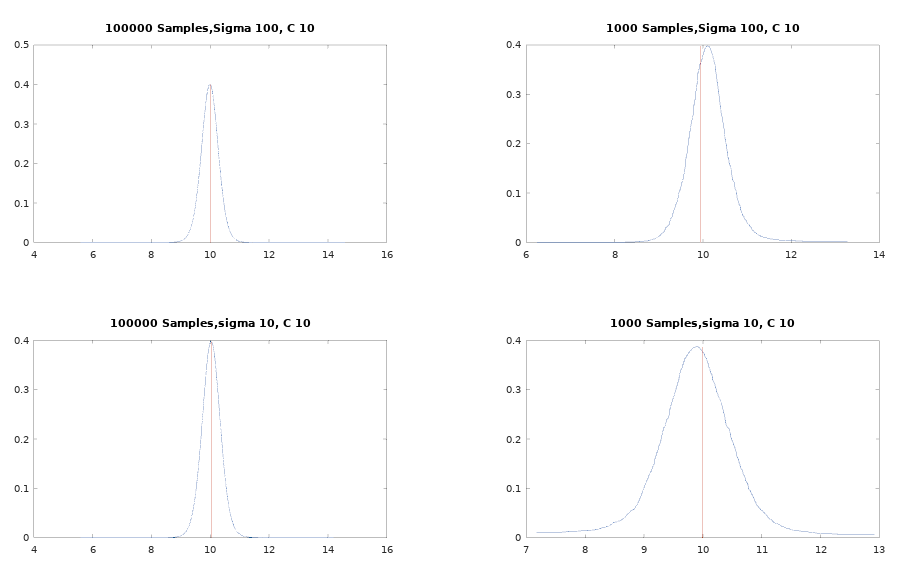
\includegraphics[width=1\linewidth]{files/curves}
	\caption{Distributions with different sample sizes and variance.}
	\label{img:curves}
\end{figure}